% Slides for 2024-04-12
% To create a slide, use the following:
% \begin{frame}{TITLE}
%     BODY
% \end{frame}

% To create a slide with a bullet list, use the following:
% \begin{frame}{TITLE}
%     \begin{itemize}
%         \item ITEM 1
%         \item ITEM 2
%     \end{itemize}    
% \end{frame}

% To create a slide with numbered list, use the following:
% \begin{frame}{TITLE}
%     \begin{enumerate}
%         \item ITEM 1
%         \item ITEM 2
%     \end{enumerate}
% \end{frame}

% To create a slide with a graphic:
% 1. Add the graphic to this folder (named picture.png)
% 2. Use the following:
% \begin{frame}{TITLE}
%     \centering
%     \includegraphics[height=0.7\textheight,width=0.7\textwidth,keepaspectratio]{picture.png}
% \end{frame}

% To create a slide with two columns, use the following:
% \begin{frame}{TITLE}
%     \begin{columns}
%         \begin{column}{0.5\textwidth}
%             COLUMN 1 BODY
%         \end{column}
%         \begin{column}{0.5\textwidth}
%             COLUMN 2 BODY
%         \end{column}
%     \end{columns}
% \end{frame}

\begin{frame}{Documentation and Such}
    Towards docker-compose and usability
\end{frame}

\begin{frame}{Refactoring User Requests}
    Band-specific sources 
    \begin{itemize}
        \item RGB
        \item NIR
    \end{itemize}    
\end{frame}


\begin{frame}{AWS Deployment Steps}
    Stripped back containers deployed
\end{frame}

\begin{frame}{Docker Compose Dev Fully Functioning}
     \centering
     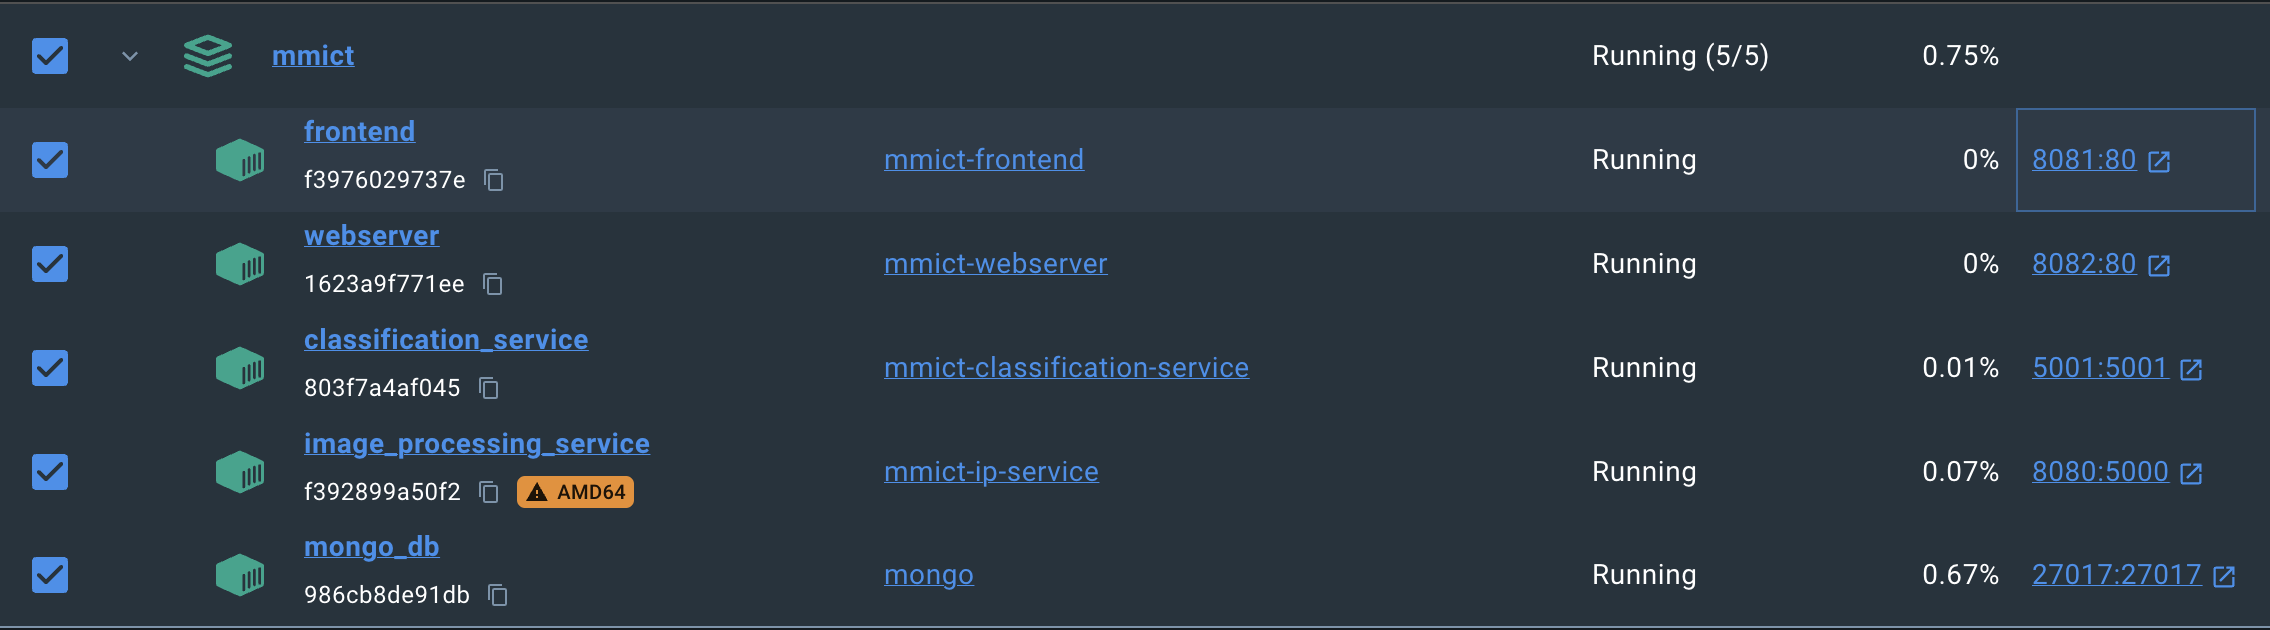
\includegraphics[height=0.7\textheight,width=0.7\textwidth,keepaspectratio]{images/MM4.png}
     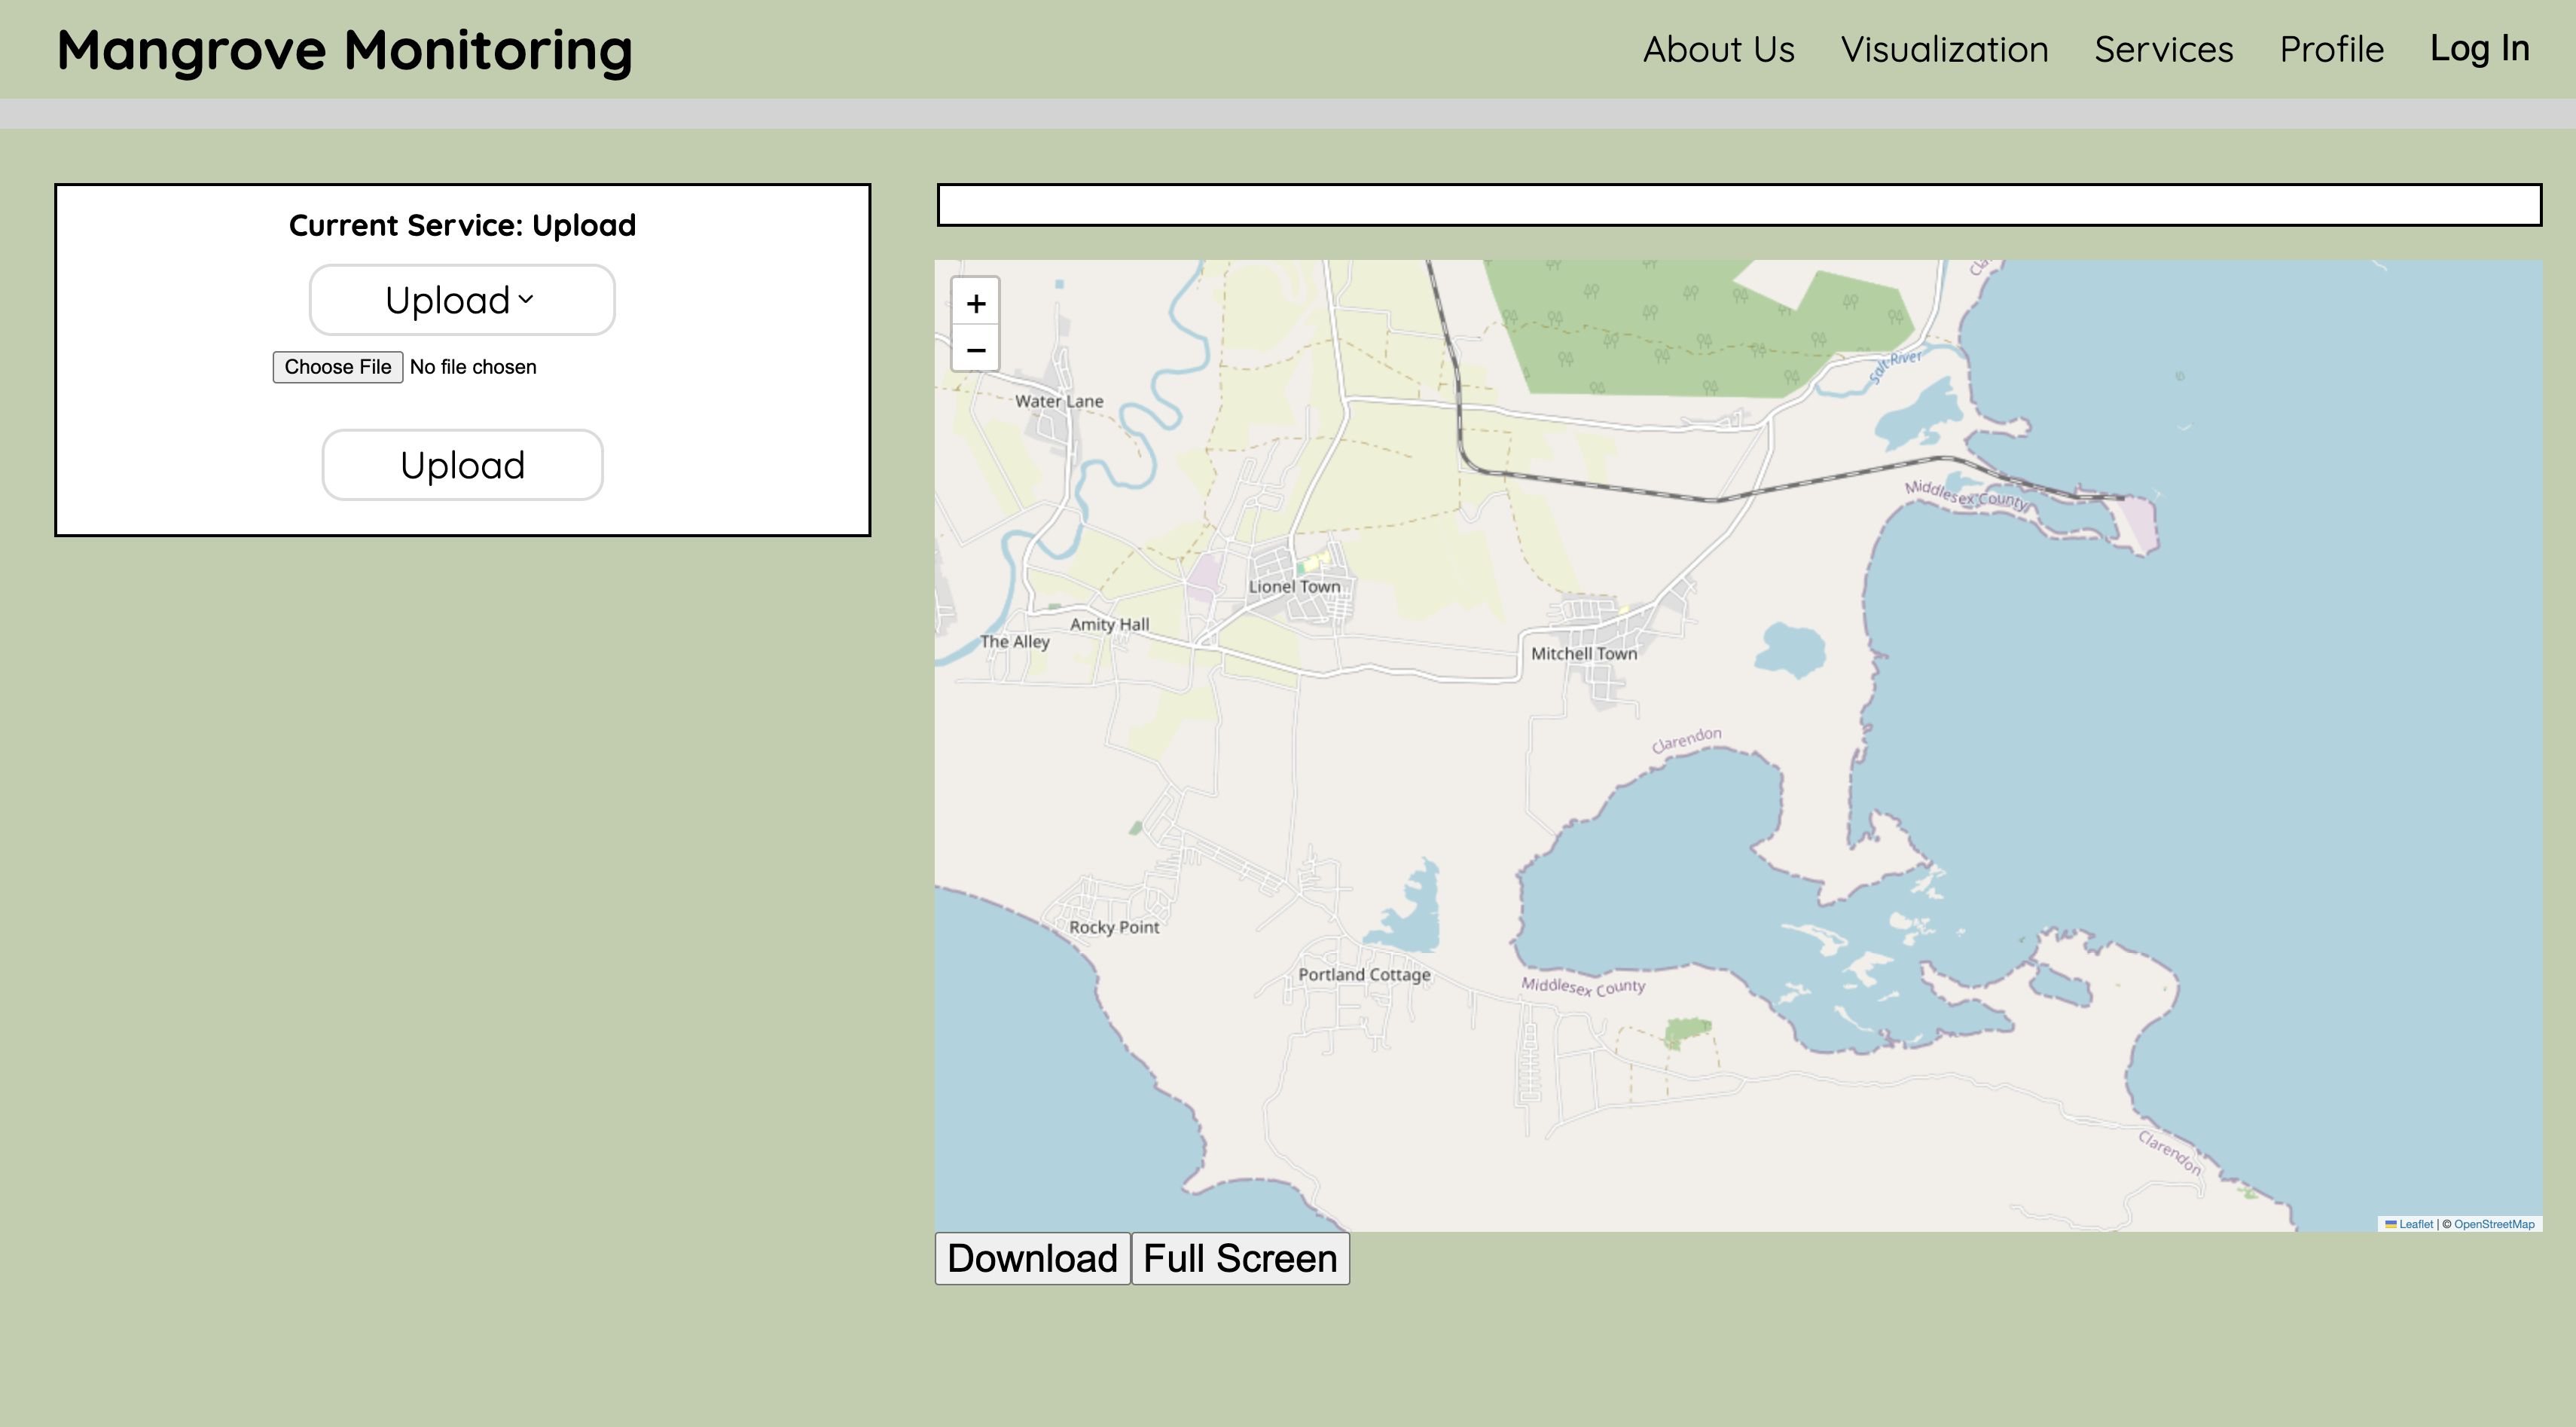
\includegraphics[height=0.7\textheight,width=0.7\textwidth,keepaspectratio]{images/MM5.png}
\end{frame}

\begin{frame}{Normalized Satellite Data}
     \centering
     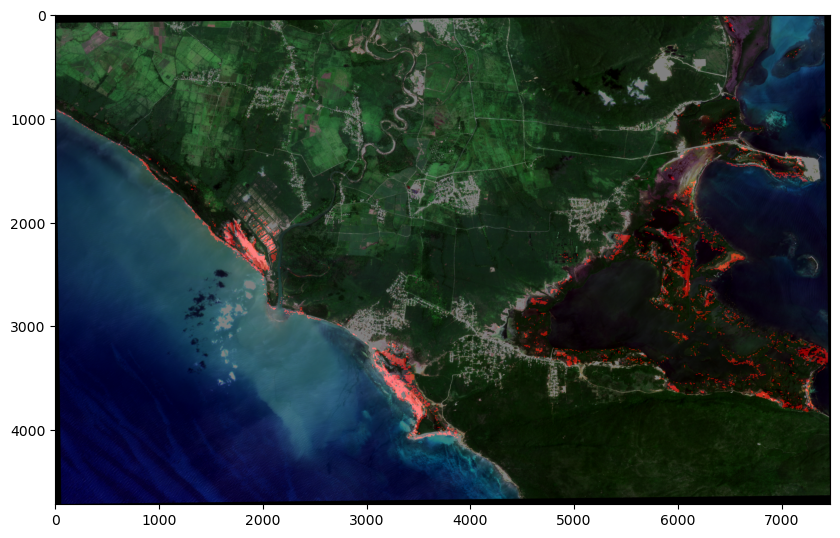
\includegraphics[height=0.7\textheight,width=0.7\textwidth,keepaspectratio]{images/MM3.png}
\end{frame}

\begin{frame}{Mask Works?}
     \centering
     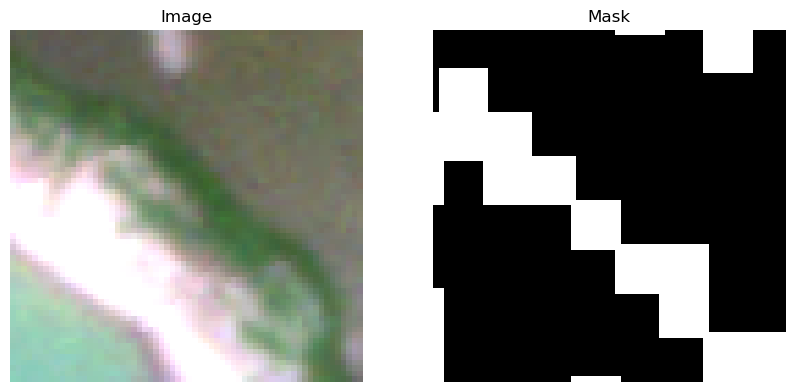
\includegraphics[height=0.7\textheight,width=0.7\textwidth,keepaspectratio]{images/MM1.png}
     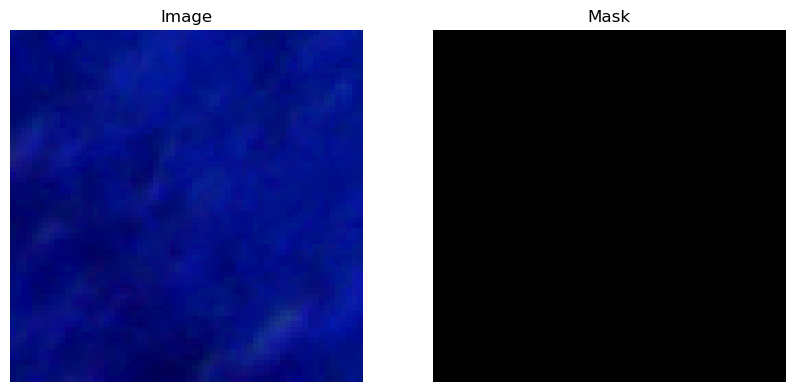
\includegraphics[height=0.7\textheight,width=0.7\textwidth,keepaspectratio]{images/MM2.png}
\end{frame}
